\documentclass[10pt,a4paper]{article}
\usepackage[utf8]{inputenc}
\usepackage[T1]{fontenc}
\usepackage{lmodern}
\usepackage[margin=1.5cm, top=1.4cm, bottom=1.4cm]{geometry}
\usepackage{hyperref}
\usepackage{enumitem}
\usepackage{titlesec}
\usepackage{xcolor}
\usepackage{graphicx}

\definecolor{accent}{HTML}{00686E}
\hypersetup{colorlinks=true, urlcolor=accent, linkcolor=accent}
\pagenumbering{arabic}
\setlength{\parindent}{0pt}

\titleformat{\section}{\large\bfseries\color{accent}}{}{0em}{}[\vspace{-0.6em}\rule{\textwidth}{0.8pt}]
\titlespacing{\section}{0pt}{7pt}{4pt}

\newcommand{\role}[4]{%
  \textbf{#1} \hfill \textbf{#2}\\[1pt]%
  \textit{#3} \hfill \textit{#4}\\[2pt]%
}
\setlist[itemize]{leftmargin=1.2em, itemsep=1.5pt, topsep=2pt, parsep=0pt}

\begin{document}

% ================= HEADER =================
\begin{minipage}[c]{0.80\textwidth}
  {\Huge\bfseries Prabhavit Gupta}\\[3pt]
  {\color{accent}\large AI Architect: Generative AI, RAG Systems \& Enterprise Public Sector IT}\\[6pt]
  {\footnotesize +39 351 610 7807 ~$\vert$~
  \href{mailto:prabhavitg@gmail.com}{prabhavitg@gmail.com} ~$\vert$~
  \href{https://www.linkedin.com/in/prabhavit/}{linkedin.com/in/prabhavit} ~$\vert$~
  \href{https://github.com/prab-gupta}{github.com/prab-gupta} ~$\vert$~
  Venice, Italy (EU Permanent Resident / Remote EU Ready)}
\end{minipage}\hfill
\begin{minipage}[c]{0.18\textwidth}
  \raggedleft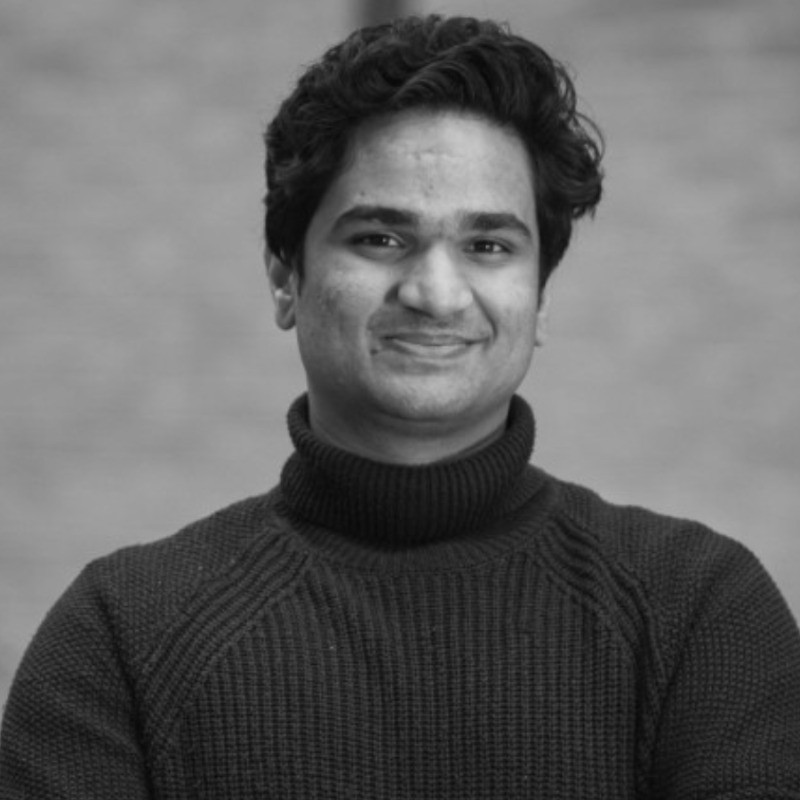
\includegraphics[width=2.0cm]{photo.jpg}
\end{minipage}
\vspace{-2pt}

% ================= SUMMARY =================
\section{Summary}
AI Systems Architect with 3 years of hands-on software and systems engineering experience designing, deploying, and operating enterprise Generative AI architectures, multi-agent pipelines, and secure RAG frameworks. Proven track record turning complex institutional requirements into robust, compliant, and auditable production AI blueprints across distributed microservices. Deep practical expertise implementing LLM evaluation harnesses, citation grounding, guardrails, and role-based data protection in alignment with European compliance standards (GDPR, EU AI Act). Holder of an EU Long-Term Residence Permit (permanent unrestricted EU work authorization across all EU member states, no sponsorship required); based in Venice, Italy and available immediately for European international projects.

% ================= TECHNICAL EXPERTISE =================
\section{Technical Expertise}
\begin{itemize}
  \item \textbf{GenAI Architecture \& Agent Systems:} Enterprise GenAI blueprints, multi-agent orchestration, tool-calling constraints, prompt engineering frameworks, human-in-the-loop approvals, structured JSON outputs, citation grounding.
  \item \textbf{RAG Pipelines \& Vector Retrievability:} Dense and sparse hybrid search (BM25 + embeddings), PostgreSQL with \texttt{pgvector}, semantic chunking, cross-encoder reranking, metadata access filtering.
  \item \textbf{AI Governance, Observability \& Quality:} Automated evaluation harnesses measuring precision, recall, and grounding against ground-truth benchmarks; audit logging, model-drift detection, and latency tracking.
  \item \textbf{Software Development \& Distributed Systems:} Python (FastAPI, asyncio, pydantic), TypeScript, Node.js, RESTful microservices, OpenAPI contracts, webhook event orchestration, Redis task queues.
  \item \textbf{Cloud Infrastructure \& CI/CD:} Docker containerization, CI/CD pipelines, Git version control, automated end-to-end integration testing with Playwright, Linux server environments.
  \item \textbf{Languages \& Work Authorization:} English (C1 Professional, fluent), Hindi (Native), Italian (Beginner). EU Long-Term Residence Permit (unrestricted EU work authorization across all EU member states, no visa sponsorship required).
\end{itemize}

% ================= EXPERIENCE =================
\section{Experience}

\role{\href{https://flowspace.co}{FlowSpace.co}}{Mar 2024 - Aug 2026}{Lead Developer \& AI Systems Architect}{London, UK (remote)}
\begin{itemize}
  \item Designed and operated production customer-facing AI agents and retrieval architectures for a platform serving 4,500+ active enterprise users, integrating live product catalogs with external APIs.
  \item Architected multi-step agent reasoning chains with strict tool execution constraints, schema validation, and human-in-the-loop checkpoints, preventing ungrounded actions in production flows.
  \item Implemented document ingestion and structured extraction pipelines with LLMs, translating unstructured partner data into validated JSON schemas.
  \item Engineered automated evaluation harnesses evaluating system accuracy, grounding, and recall against production transcripts, systematically lowering edge-case error rates.
  \item Maintained resilient TypeScript/Node.js backend microservices and PostgreSQL data models, utilizing asynchronous Redis queues to handle high-throughput query spikes.
  \item Built automated integration and regression test suites with Playwright, verifying API contracts and preventing system regressions across continuous release cycles.
\end{itemize}

\role{Urlink}{Apr 2025 - Jul 2025}{Project Manager \& Solutions Developer (Freelance)}{Barcelona, Spain (remote)}
\begin{itemize}
  \item Led technical discovery, solution architecture, and client delivery of customized web solutions and automated data processing pipelines for European client platforms.
  \item Built automated data ingestion and transformation services connecting third-party APIs to PostgreSQL databases, maintaining high data freshness and integrity.
  \item Delivered interactive functional prototypes to validate user flows and technical requirements prior to sprint execution, accelerating cycle times.
\end{itemize}

\role{Independent Technical Consultant}{Aug 2023 - Feb 2024}{AI Automation \& Integration Developer}{Venice, Italy}
\begin{itemize}
  \item Built and deployed custom LLM integrations, document retrieval prototypes, and webhook automation workflows for European enterprise clients using Python, TypeScript, and n8n.
  \item Replaced brittle manual document review workflows with automated LLM-assisted classification and extraction pipelines featuring comprehensive error handling and fallback routing.
  \item Authored technical architecture specifications, API documentation, and deployment guides to support client engineering teams in operating self-hosted workflows.
\end{itemize}

% ================= EDUCATION =================
\section{Education}
\role{Ca' Foscari University of Venice}{2020 - 2024}{BA in Philosophy, International Studies and Economics}{Venice, Italy}
\begin{itemize}
  \item Rigorous training in formal logic, analytical problem solving, systems analysis, and macroeconomic decision models.
\end{itemize}

\end{document}
